\subsection{Administrador de Desafíos}

\begin{figure}[H]
   \centering
   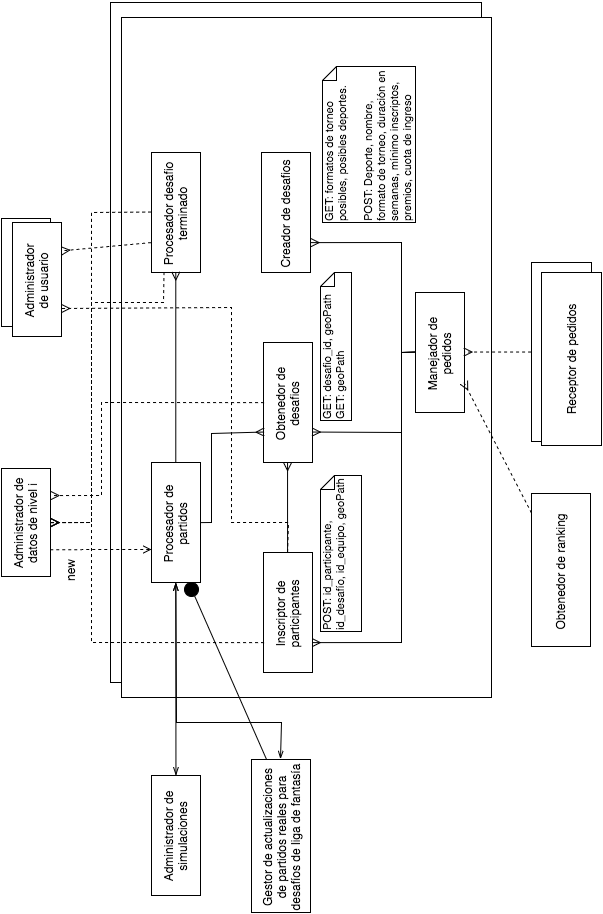
\includegraphics[height=0.95\textheight]{reentrega/imagenes/desafios-1.png}
   \caption{Zoom de Administrador de desafios.}
\end{figure}

Un administrador de desafíos se encarga de crear y mostrar desafíos, inscribir participantes y procesar (en el momento correspondiente) los partidos que componen un desafío.
Su interfaz permite:
\begin{itemize}
	\item Obtener información de un determinado desafío mediante el id_desafío y geoPath correspondiente.
	\item Obtener información de todos los desafíos abiertos de un determinado geoPath.
	\item Inscribir un participante en un desafío.
	\item Crear desafíos
	\item Ver qué tipos de desafíos es posible crear
\end{itemize}

Para entender su funcionamiento hagamos zoom en cada uno de los componentes:

% SEGUNDA FIGURA
\begin{figure}[H]
   \centering
   \includegraphics[width=\textwidth]{reentrega/imagenes/desafios-2.png}
   \caption{Zoom de Inscriptor de participantes.}
\end{figure}

Inscriptor de participantes: Dado un pedido de inscripción con id_desafio, id_usuario, equipo_id y geoPath, el procesador de solicitudes de inscripcion de desafíos llama al
obtenedor de desafios para conocer cuál es la cuota necesaria para anotarse en el desafío con id_desafio. Luego, hace un request al validador de inscripción pasándole el id_usuario, cuota
necesaria para anotarse, id_equipo y geoPath. El validador de inscripción verifica que el id_equipo sea un equipo de id_usuario y que, además, el usuario disponga de las fichas necesarias
para anotarse al desafío. Si el validador valida que la información es correcta entonces el procesador de solicitudes llama al cobrador de inscripción que fowardea el pedido al administrador de usuarios para que se descuente la cuota del usuario que se quiere inscribir. Luego, el inscriptor de usuario inscribe al usuario en el desafio llamando al administrador
de datos que persiste esta información.

% TERCER FIGURA
\begin{figure}[H]
  \centering
  \includegraphics[width=\textwidth]{reentrega/imagenes/desafios-3.png}
  \caption{Zoom Creador de desafios.}
\end{figure}

Creador de desafios: El creador de desafíos se encarga, como su nombre indica, de crear desafíos y de consultar qué tipos de desafíos se pueden crear. Para ello, utiliza el administrador de
datos.

% CUARTA FIGURA
\begin{figure}[H]
  \centering
  \includegraphics[width=\textwidth]{reentrega/imagenes/desafios-4.png}
  \caption{Zoom Obtenedor de desafíos.}
\end{figure}

Obtenedor de desafíos: el recolector de detalles de desafío devuelve el estado de un desafio especifico (o todos los del geoPath solicitado si no se especificó un desafío en particualar): si está abierto a inscripciones, si se esta jugando o si está terminado, y todos los detalles asociados: premios, cuota de inscripción, tipo de desafío, formato de torneo o fechas que se juegan, etc. El recolector de ranking obtiene el ranking para un determinado desafío.

% QUINTA FIGURA

\begin{figure}[H]
  \centering
  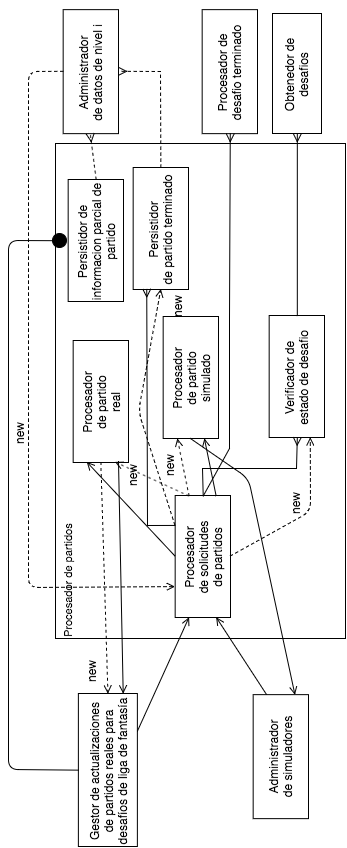
\includegraphics[height=0.95\textheight]{reentrega/imagenes/desafios-5.png}
  \caption{Zoom Procesador de partidos.}
\end{figure}

Procesador de partidos:
Flujo para el procesamiento de un partido simulado: El administrador de datos dispara un trigger al procesador de solicitudes de partidos para que este procese el partido
que acaba de comenzar. Como se trata de un partido simulado, el procesador de solicitudes llama al procesador de partido simulado. Este, le avisa el administrador de simuladores que la simulación debe comenzar. Una vez finalizada la misma, el administrador de simuladores le informa al procesador de solicitudes que el partido finalizó y cómo (quién ganó). Luego, persistidor de partido terminado persiste en el administrador de datos toda la información relacionada al partido que acaba de finalizar.
En caso de que el partido fuera el último del desafío (condición que es verificada por el Verificador de estado de desafío), se llama al procesador de desafío terminado para finalizar el desafío.
Flujo para el procesamiento de un partido real: Parecido al flujo antes mencionado pero con algunas diferencias: si el partido que se va a ejecutar se encuentra en más de un desafío solo se dispara un trigger. Queda bajo responsabilidad del procesador de partidos persisitir el resultado de dicho partido en cada desafío que tiene el partido. Además, a diferencia de la simulación, el gestor de actualizaciones de partidos reales otorga información del partido minuto a minuto por lo cual se realizan actualizaciones periódicas del partido en el administrador de datos. Una vez finalizado el encuentro, el gestor notifica al procesador de solicitudes de partidos para que persista la finalización del mismo. El flujo aquí es igual al caso simulado.

% SEXTA FIGURA
\begin{figure}[H]
  \centering
  \includegraphics[width=\textwidth]{reentrega/imagenes/desafios-6.png}
  \caption{Zoom Procesador de desafio terminado.}
\end{figure}

Procesador de desafío terminado: dado un pedido de finalizar un desafío, el receptor de desafios terminados llama al persistidor de cambio de estado de desafío para finalizar el desafío.
Luego, el entregador de premios calcula los puntos obtenidos para cada usuario y fowardea al administrador de usuarios para que persista dichos puntos.
